% Options for packages loaded elsewhere
\PassOptionsToPackage{unicode}{hyperref}
\PassOptionsToPackage{hyphens}{url}
\PassOptionsToPackage{dvipsnames,svgnames,x11names}{xcolor}
%
\documentclass[
  letterpaper,
  DIV=11,
  numbers=noendperiod]{scrreprt}
\usepackage{amsmath,amssymb}
\usepackage{lmodern}
\usepackage{iftex}
\ifPDFTeX
  \usepackage[T1]{fontenc}
  \usepackage[utf8]{inputenc}
  \usepackage{textcomp} % provide euro and other symbols
\else % if luatex or xetex
  \usepackage{unicode-math}
  \defaultfontfeatures{Scale=MatchLowercase}
  \defaultfontfeatures[\rmfamily]{Ligatures=TeX,Scale=1}
\fi
% Use upquote if available, for straight quotes in verbatim environments
\IfFileExists{upquote.sty}{\usepackage{upquote}}{}
\IfFileExists{microtype.sty}{% use microtype if available
  \usepackage[]{microtype}
  \UseMicrotypeSet[protrusion]{basicmath} % disable protrusion for tt fonts
}{}
\makeatletter
\@ifundefined{KOMAClassName}{% if non-KOMA class
  \IfFileExists{parskip.sty}{%
    \usepackage{parskip}
  }{% else
    \setlength{\parindent}{0pt}
    \setlength{\parskip}{6pt plus 2pt minus 1pt}}
}{% if KOMA class
  \KOMAoptions{parskip=half}}
\makeatother
\usepackage{xcolor}
\IfFileExists{xurl.sty}{\usepackage{xurl}}{} % add URL line breaks if available
\IfFileExists{bookmark.sty}{\usepackage{bookmark}}{\usepackage{hyperref}}
\hypersetup{
  pdftitle={Example Jupyter Notebook},
  colorlinks=true,
  linkcolor={blue},
  filecolor={Maroon},
  citecolor={Blue},
  urlcolor={Blue},
  pdfcreator={LaTeX via pandoc}}
\urlstyle{same} % disable monospaced font for URLs
\usepackage{color}
\usepackage{fancyvrb}
\newcommand{\VerbBar}{|}
\newcommand{\VERB}{\Verb[commandchars=\\\{\}]}
\DefineVerbatimEnvironment{Highlighting}{Verbatim}{commandchars=\\\{\}}
% Add ',fontsize=\small' for more characters per line
\usepackage{framed}
\definecolor{shadecolor}{RGB}{241,243,245}
\newenvironment{Shaded}{\begin{snugshade}}{\end{snugshade}}
\newcommand{\AlertTok}[1]{\textcolor[rgb]{0.68,0.00,0.00}{#1}}
\newcommand{\AnnotationTok}[1]{\textcolor[rgb]{0.37,0.37,0.37}{#1}}
\newcommand{\AttributeTok}[1]{\textcolor[rgb]{0.00,0.48,0.65}{#1}}
\newcommand{\BaseNTok}[1]{\textcolor[rgb]{0.68,0.00,0.00}{#1}}
\newcommand{\BuiltInTok}[1]{\textcolor[rgb]{0.00,0.48,0.65}{#1}}
\newcommand{\CharTok}[1]{\textcolor[rgb]{0.13,0.47,0.30}{#1}}
\newcommand{\CommentTok}[1]{\textcolor[rgb]{0.37,0.37,0.37}{#1}}
\newcommand{\CommentVarTok}[1]{\textcolor[rgb]{0.37,0.37,0.37}{\textit{#1}}}
\newcommand{\ConstantTok}[1]{\textcolor[rgb]{0.56,0.35,0.01}{#1}}
\newcommand{\ControlFlowTok}[1]{\textcolor[rgb]{0.00,0.48,0.65}{#1}}
\newcommand{\DataTypeTok}[1]{\textcolor[rgb]{0.68,0.00,0.00}{#1}}
\newcommand{\DecValTok}[1]{\textcolor[rgb]{0.68,0.00,0.00}{#1}}
\newcommand{\DocumentationTok}[1]{\textcolor[rgb]{0.37,0.37,0.37}{\textit{#1}}}
\newcommand{\ErrorTok}[1]{\textcolor[rgb]{0.68,0.00,0.00}{#1}}
\newcommand{\ExtensionTok}[1]{\textcolor[rgb]{0.00,0.48,0.65}{#1}}
\newcommand{\FloatTok}[1]{\textcolor[rgb]{0.68,0.00,0.00}{#1}}
\newcommand{\FunctionTok}[1]{\textcolor[rgb]{0.28,0.35,0.67}{#1}}
\newcommand{\ImportTok}[1]{\textcolor[rgb]{0.00,0.48,0.65}{#1}}
\newcommand{\InformationTok}[1]{\textcolor[rgb]{0.37,0.37,0.37}{#1}}
\newcommand{\KeywordTok}[1]{\textcolor[rgb]{0.00,0.48,0.65}{#1}}
\newcommand{\NormalTok}[1]{\textcolor[rgb]{0.00,0.48,0.65}{#1}}
\newcommand{\OperatorTok}[1]{\textcolor[rgb]{0.37,0.37,0.37}{#1}}
\newcommand{\OtherTok}[1]{\textcolor[rgb]{0.00,0.48,0.65}{#1}}
\newcommand{\PreprocessorTok}[1]{\textcolor[rgb]{0.68,0.00,0.00}{#1}}
\newcommand{\RegionMarkerTok}[1]{\textcolor[rgb]{0.00,0.48,0.65}{#1}}
\newcommand{\SpecialCharTok}[1]{\textcolor[rgb]{0.37,0.37,0.37}{#1}}
\newcommand{\SpecialStringTok}[1]{\textcolor[rgb]{0.13,0.47,0.30}{#1}}
\newcommand{\StringTok}[1]{\textcolor[rgb]{0.13,0.47,0.30}{#1}}
\newcommand{\VariableTok}[1]{\textcolor[rgb]{0.07,0.07,0.07}{#1}}
\newcommand{\VerbatimStringTok}[1]{\textcolor[rgb]{0.13,0.47,0.30}{#1}}
\newcommand{\WarningTok}[1]{\textcolor[rgb]{0.37,0.37,0.37}{\textit{#1}}}
\usepackage{longtable,booktabs,array}
\usepackage{calc} % for calculating minipage widths
% Correct order of tables after \paragraph or \subparagraph
\usepackage{etoolbox}
\makeatletter
\patchcmd\longtable{\par}{\if@noskipsec\mbox{}\fi\par}{}{}
\makeatother
% Allow footnotes in longtable head/foot
\IfFileExists{footnotehyper.sty}{\usepackage{footnotehyper}}{\usepackage{footnote}}
\makesavenoteenv{longtable}
\usepackage{graphicx}
\makeatletter
\def\maxwidth{\ifdim\Gin@nat@width>\linewidth\linewidth\else\Gin@nat@width\fi}
\def\maxheight{\ifdim\Gin@nat@height>\textheight\textheight\else\Gin@nat@height\fi}
\makeatother
% Scale images if necessary, so that they will not overflow the page
% margins by default, and it is still possible to overwrite the defaults
% using explicit options in \includegraphics[width, height, ...]{}
\setkeys{Gin}{width=\maxwidth,height=\maxheight,keepaspectratio}
% Set default figure placement to htbp
\makeatletter
\def\fps@figure{htbp}
\makeatother
\setlength{\emergencystretch}{3em} % prevent overfull lines
\providecommand{\tightlist}{%
  \setlength{\itemsep}{0pt}\setlength{\parskip}{0pt}}
\setcounter{secnumdepth}{5}
\KOMAoption{captions}{tableheading}
\makeatletter
\makeatother
\makeatletter
\@ifpackageloaded{caption}{}{\usepackage{caption}}
\AtBeginDocument{%
\renewcommand*\contentsname{Table of contents}
\renewcommand*\listfigurename{List of Figures}
\renewcommand*\listtablename{List of Tables}
\renewcommand*\figurename{Figure}
\renewcommand*\tablename{Table}
}
\@ifpackageloaded{float}{}{\usepackage{float}}
\floatstyle{ruled}
\@ifundefined{c@chapter}{\newfloat{codelisting}{h}{lop}}{\newfloat{codelisting}{h}{lop}[chapter]}
\floatname{codelisting}{Listing}
\newcommand*\listoflistings{\listof{codelisting}{List of Listings}}
\makeatother
\makeatletter
\@ifpackageloaded{caption}{}{\usepackage{caption}}
\@ifpackageloaded{subcaption}{}{\usepackage{subcaption}}
\makeatother
\makeatletter
\makeatother
\ifLuaTeX
  \usepackage{selnolig}  % disable illegal ligatures
\fi

\title{Example Jupyter Notebook}
\usepackage{etoolbox}
\makeatletter
\providecommand{\subtitle}[1]{% add subtitle to \maketitle
  \apptocmd{\@title}{\par {\large #1 \par}}{}{}
}
\makeatother
\subtitle{The R4DS Online Learning Community}
\author{}
\date{}

\begin{document}
\maketitle

\renewcommand*\contentsname{Table of contents}
{
\hypersetup{linkcolor=}
\setcounter{tocdepth}{2}
\tableofcontents
}
\hypertarget{welcome}{%
\section*{Welcome}\label{welcome}}
\addcontentsline{toc}{section}{Welcome}

This is a companion for the book
\href{https://dabeaz-course.github.io/practical-python/}{Practical
Python Programming} by David Beazley.

This website is being developed by the
\href{https://rfordatasci.com/}{R4DS Online Learning Community}. Follow
along and \href{https://r4ds.io/join}{join the community} to
participate.

This companion follows the \href{https://r4ds.io/conduct}{R4DS Online
Learning Community Code of Conduct}.

\hypertarget{book-club-meetings}{%
\section*{Book club meetings}\label{book-club-meetings}}
\addcontentsline{toc}{section}{Book club meetings}

\begin{itemize}
\item
  Each week, a volunteer will present a chapter from the book.

  \begin{itemize}
  \tightlist
  \item
    This is the best way to learn the material.
  \end{itemize}
\item
  Presentations will usually consist of a review of the material, a
  discussion, and/or a demonstration of the principles presented in that
  chapter.
\item
  More information about how to present is available in the GitHub repo.
\item
  Presentations will be recorded and will be available on the
  \href{https://r4ds.io/youtube}{R4DS Online Learning Community YouTube
  Channel}.
\end{itemize}

\part{1. Introduction to Python}

\hypertarget{learning-objectives}{%
\subsubsection*{Learning Objectives}\label{learning-objectives}}
\addcontentsline{toc}{subsubsection}{Learning Objectives}

\begin{itemize}
\tightlist
\item
  Learning objective 1
\end{itemize}

\hypertarget{notes}{%
\chapter*{Notes}\label{notes}}
\addcontentsline{toc}{chapter}{Notes}

\hypertarget{slides}{%
\section*{Slides}\label{slides}}
\addcontentsline{toc}{section}{Slides}

{[}insert slides{]}

\hypertarget{notes-1}{%
\section*{Notes}\label{notes-1}}
\addcontentsline{toc}{section}{Notes}

{[}insert notes{]}

\hypertarget{video}{%
\chapter*{Video}\label{video}}
\addcontentsline{toc}{chapter}{Video}

\hypertarget{cohort-01}{%
\section*{Cohort 01}\label{cohort-01}}
\addcontentsline{toc}{section}{Cohort 01}

{[}insert video here{]}

\part{2. Working with Data}

\hypertarget{learning-objectives-1}{%
\subsubsection*{Learning Objectives}\label{learning-objectives-1}}
\addcontentsline{toc}{subsubsection}{Learning Objectives}

\begin{itemize}
\tightlist
\item
  Learning objective 1
\end{itemize}

\hypertarget{notes-2}{%
\chapter*{Notes}\label{notes-2}}
\addcontentsline{toc}{chapter}{Notes}

\hypertarget{slides-1}{%
\section*{Slides}\label{slides-1}}
\addcontentsline{toc}{section}{Slides}

{[}insert slides{]}

\hypertarget{notes-3}{%
\section*{Notes}\label{notes-3}}
\addcontentsline{toc}{section}{Notes}

{[}insert notes{]}

\hypertarget{video-1}{%
\chapter*{Video}\label{video-1}}
\addcontentsline{toc}{chapter}{Video}

\hypertarget{cohort-01-1}{%
\section*{Cohort 01}\label{cohort-01-1}}
\addcontentsline{toc}{section}{Cohort 01}

{[}insert video here{]}

\part{3. Program Organization}

\hypertarget{notes-4}{%
\chapter{Notes}\label{notes-4}}

\hypertarget{video-2}{%
\chapter{Video}\label{video-2}}

\part{Examples}

\hypertarget{example-quarto-document}{%
\chapter{Example Quarto Document}\label{example-quarto-document}}

\hypertarget{quarto}{%
\section{Quarto}\label{quarto}}

Quarto enables you to weave together content and executable code into a
finished document. To learn more about Quarto see
\url{https://quarto.org}.

\hypertarget{running-code}{%
\section{Running Code}\label{running-code}}

When you click the \textbf{Render} button a document will be generated
that includes both content and the output of embedded code. You can
embed code like this:

\begin{Shaded}
\begin{Highlighting}[]
\DecValTok{1} \OperatorTok{+} \DecValTok{1}
\end{Highlighting}
\end{Shaded}

\begin{verbatim}
2
\end{verbatim}

You can add options to executable code like this

\begin{verbatim}
4
\end{verbatim}

The \texttt{echo:\ false} option disables the printing of code (only
output is displayed).

\hypertarget{example-jupyter-notebook}{%
\chapter{Example Jupyter Notebook}\label{example-jupyter-notebook}}

\hypertarget{numpy}{%
\section{NumPy}\label{numpy}}

\begin{Shaded}
\begin{Highlighting}[]
\ImportTok{import}\NormalTok{ numpy }\ImportTok{as}\NormalTok{ np}
\NormalTok{a }\OperatorTok{=}\NormalTok{ np.arange(}\DecValTok{15}\NormalTok{).reshape(}\DecValTok{3}\NormalTok{, }\DecValTok{5}\NormalTok{)}
\NormalTok{a}
\end{Highlighting}
\end{Shaded}

\begin{verbatim}
array([[ 0,  1,  2,  3,  4],
       [ 5,  6,  7,  8,  9],
       [10, 11, 12, 13, 14]])
\end{verbatim}

\hypertarget{matplotlib}{%
\section{Matplotlib}\label{matplotlib}}

\begin{Shaded}
\begin{Highlighting}[]
\ImportTok{import}\NormalTok{ matplotlib.pyplot }\ImportTok{as}\NormalTok{ plt}

\NormalTok{fig }\OperatorTok{=}\NormalTok{ plt.figure()}
\NormalTok{x }\OperatorTok{=}\NormalTok{ np.arange(}\DecValTok{10}\NormalTok{)}
\NormalTok{y }\OperatorTok{=} \FloatTok{2.5} \OperatorTok{*}\NormalTok{ np.sin(x }\OperatorTok{/} \DecValTok{20} \OperatorTok{*}\NormalTok{ np.pi)}
\NormalTok{yerr }\OperatorTok{=}\NormalTok{ np.linspace(}\FloatTok{0.05}\NormalTok{, }\FloatTok{0.2}\NormalTok{, }\DecValTok{10}\NormalTok{)}

\NormalTok{plt.errorbar(x, y }\OperatorTok{+} \DecValTok{3}\NormalTok{, yerr}\OperatorTok{=}\NormalTok{yerr, label}\OperatorTok{=}\StringTok{\textquotesingle{}both limits (default)\textquotesingle{}}\NormalTok{)}
\NormalTok{plt.errorbar(x, y }\OperatorTok{+} \DecValTok{2}\NormalTok{, yerr}\OperatorTok{=}\NormalTok{yerr, uplims}\OperatorTok{=}\VariableTok{True}\NormalTok{, label}\OperatorTok{=}\StringTok{\textquotesingle{}uplims=True\textquotesingle{}}\NormalTok{)}
\NormalTok{plt.errorbar(x, y }\OperatorTok{+} \DecValTok{1}\NormalTok{, yerr}\OperatorTok{=}\NormalTok{yerr, uplims}\OperatorTok{=}\VariableTok{True}\NormalTok{, lolims}\OperatorTok{=}\VariableTok{True}\NormalTok{,}
\NormalTok{             label}\OperatorTok{=}\StringTok{\textquotesingle{}uplims=True, lolims=True\textquotesingle{}}\NormalTok{)}

\NormalTok{upperlimits }\OperatorTok{=}\NormalTok{ [}\VariableTok{True}\NormalTok{, }\VariableTok{False}\NormalTok{] }\OperatorTok{*} \DecValTok{5}
\NormalTok{lowerlimits }\OperatorTok{=}\NormalTok{ [}\VariableTok{False}\NormalTok{, }\VariableTok{True}\NormalTok{] }\OperatorTok{*} \DecValTok{5}
\NormalTok{plt.errorbar(x, y, yerr}\OperatorTok{=}\NormalTok{yerr, uplims}\OperatorTok{=}\NormalTok{upperlimits, lolims}\OperatorTok{=}\NormalTok{lowerlimits,}
\NormalTok{             label}\OperatorTok{=}\StringTok{\textquotesingle{}subsets of uplims and lolims\textquotesingle{}}\NormalTok{)}

\NormalTok{plt.legend(loc}\OperatorTok{=}\StringTok{\textquotesingle{}lower right\textquotesingle{}}\NormalTok{)}
\NormalTok{plt.show(fig)}
\end{Highlighting}
\end{Shaded}

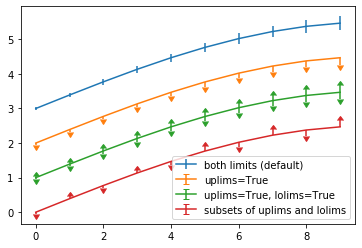
\includegraphics{./example_python_files/figure-pdf/cell-3-output-1.png}

\appendix
\addcontentsline{toc}{part}{Appendices}

\hypertarget{how-to-add-to-the-book}{%
\chapter*{How to add to the book}\label{how-to-add-to-the-book}}
\addcontentsline{toc}{chapter}{How to add to the book}

\hypertarget{set-up-quarto}{%
\section*{Set up Quarto}\label{set-up-quarto}}
\addcontentsline{toc}{section}{Set up Quarto}

This book is made with \href{https://quarto.org/}{Quarto}. Please see
the \href{https://quarto.org/docs/get-started/}{Get Started} chapter of
the Quarto documentation to learn how to install and run Quarto in your
IDE.

\hypertarget{add-to-book}{%
\section*{Add to book}\label{add-to-book}}
\addcontentsline{toc}{section}{Add to book}

Once you have everything set up, forked the repo, and cloned to your
computer, you can add a new chapter to the book:

\begin{itemize}
\tightlist
\item
  In the \texttt{\_quarto.yml} file, under \texttt{chapters}, add a part
  with your chapter like so:
\end{itemize}

\begin{Shaded}
\begin{Highlighting}[]
\AttributeTok{  }\KeywordTok{{-}}\AttributeTok{ }\FunctionTok{part}\KeywordTok{:}\AttributeTok{ 01\_main.qmd}
\AttributeTok{      }\FunctionTok{chapters}\KeywordTok{:}\AttributeTok{ }
\AttributeTok{      }\KeywordTok{{-}}\AttributeTok{ 01\_notes.qmd}
\AttributeTok{      }\KeywordTok{{-}}\AttributeTok{ 01\_video.qmd}
\end{Highlighting}
\end{Shaded}

Create the corresponding files in the main directory. You can use
\texttt{.qmd} or \texttt{.ipynb} files that run computations if you
would like, or just plain \texttt{.md} files. Check out the files under
Examples to see how they are done.

\hypertarget{render-the-book}{%
\section*{Render the book}\label{render-the-book}}
\addcontentsline{toc}{section}{Render the book}

Once you have added and edited your files, don't forget to render the
book:

\begin{Shaded}
\begin{Highlighting}[]
\ExtensionTok{quarto}\NormalTok{ render}
\end{Highlighting}
\end{Shaded}

\hypertarget{push-up-to-github}{%
\section*{Push up to GitHub}\label{push-up-to-github}}
\addcontentsline{toc}{section}{Push up to GitHub}

Push your changes to your forked repo and then create a pull request for
the R4DS admins to merge your changes.

\end{document}
